\documentclass{standalone}

\usepackage{tikz}
    \usetikzlibrary{calc}
    
\usepackage{bm}

\begin{document}
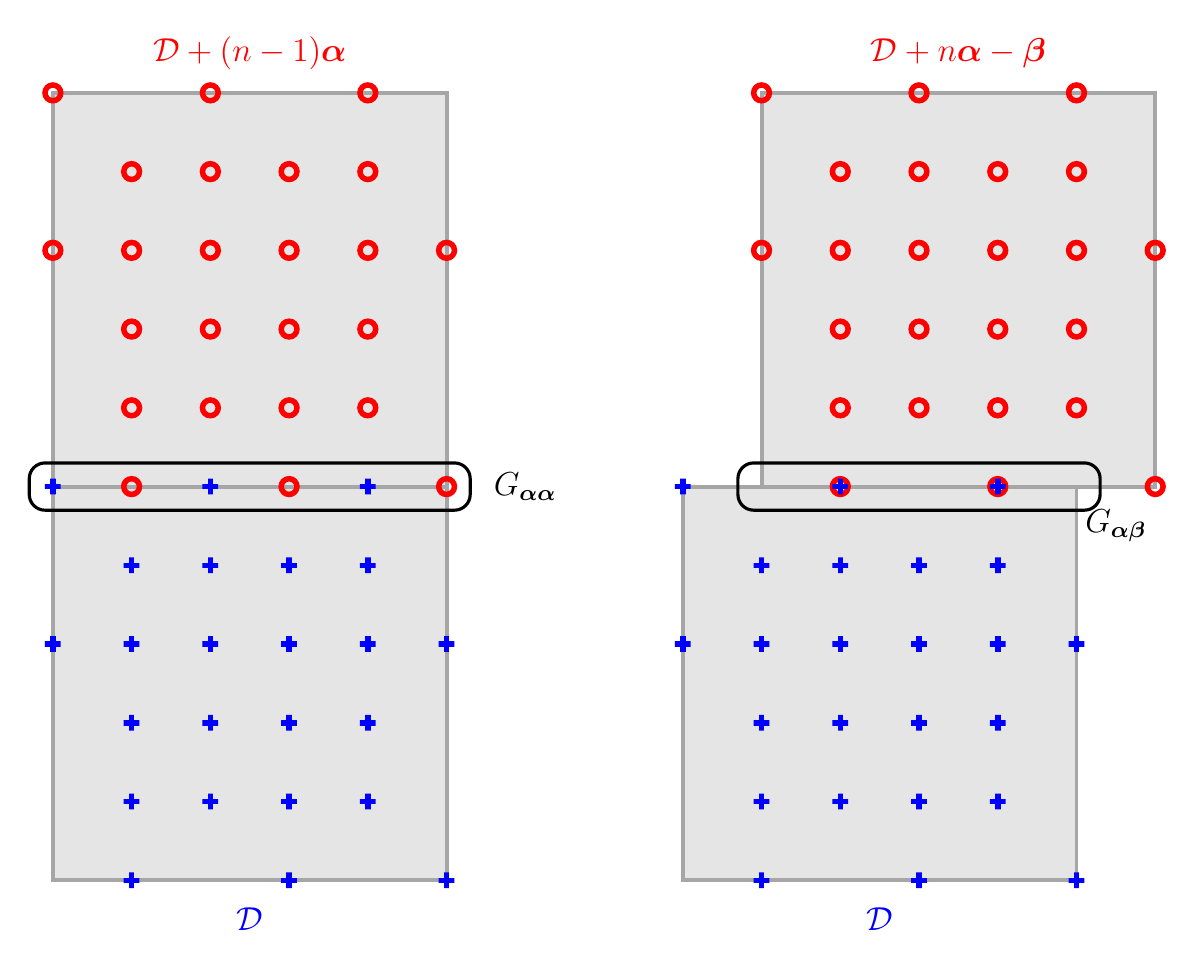
\begin{tikzpicture}
    % \draw[help lines] (0,0) grid (15,3);
    \draw[black!35, line width=0.5mm, fill=black!10] 
    	 (0,0) rectangle (5,5)
    	 (0,5) rectangle (5,10)
    	 (8,0) rectangle (13,5)
    	 (9,5) rectangle (14,10);
    \foreach \x in % green
        {(1,0), (3,0), (5,0),
         (1,1), (2,1), (3,1), (4,1),
         (1,2), (2,2), (3,2), (4,2),
         (0,3), (1,3), (2,3), (3,3), (4,3), (5,3),
         (1,4), (2,4), (3,4), (4,4),
         (0,5), (2,5), (4,5)} 
        {\draw[blue, line width=0.7mm] 
             \x++(-0.1,0) rectangle+(0.2,0)
             \x++(0,-0.1) rectangle+(0,0.2);
		  \draw[red, line width=0.7mm] 
             \x++(0,5) circle (0.1);
         \draw[blue, line width=0.7mm] 
             \x++(8,0)++(-0.1,0) rectangle+(0.2,0)
             \x++(8,0)++(0,-0.1) rectangle+(0,0.2);
		  \draw[red, line width=0.7mm] 
             \x++(9,5) circle (0.1);}
		 \node[blue] at (2.5,-0.5) {\large $\mathcal{D}$};
		 \node[red] at (2.5,10.5) {\large $\mathcal{D}+(n-1)\bm{\alpha}$};
		 \node[blue] at (10.5,-0.5) {\large $\mathcal{D}$};
		 \node[red]  at (11.5,10.5) {\large $\mathcal{D}+n\bm{\alpha}-\bm{\beta}$};
		 \node at (6,5) {\large $G_{\bm{\alpha\alpha}}$};
		 \node at (13.5,4.5) {\large $G_{\bm{\alpha\beta}}$};
		 \draw[black, line width=0.4mm, rounded corners=2mm]
    	     (-0.3,4.7) rectangle (5.3,5.3)
    	     (8.7,4.7) rectangle (13.3,5.3);

\end{tikzpicture}
\end{document}